\documentclass{article} % For LaTeX2e
\usepackage{nips13submit_e,times}
\usepackage{hyperref}
\usepackage{url}
\usepackage[dvips]{graphicx}
%\documentstyle[nips13submit_09,times,art10]{article} % For LaTeX 2.09
\usepackage{amssymb,amsmath,mathrsfs}
\usepackage{algorithm}
\usepackage[noend]{algorithmic}
\usepackage{multicol}
\usepackage{subfig}
\graphicspath{{./eps//}}
\captionsetup{belowskip=4pt,aboveskip=4pt}

\def\algorithmicrequire{\textbf{Input:}}
\def\algorithmicensure{\textbf{Output:}}
\def\algorithmicif{\textbf{if}}
\def\algorithmicthen{\textbf{then}}
\def\algorithmicelse{\textbf{else}}
\def\algorithmicelsif{\textbf{else if}}
\def\algorithmicfor{\textbf{for}}
\def\algorithmicforall{\textbf{for all}}
\def\algorithmicdo{}
\def\algorithmicwhile{\textbf{while}}
\def\algorithmicrepeat{\textbf{repeat}}
\def\algorithmicuntil{\textbf{until}}
\def\algorithmicloop{\textbf{loop}}
\def\algorithmicgoto{\textbf{goto step}}
\def\algorithmicreturn{\textbf{return}}
\newcommand{\LINEIF}[2]{%
    \STATE\algorithmicif\ {#1}\ \algorithmicthen\ {#2} %
}
\newcommand{\GOTO}[1]{%
    \algorithmicgoto\ {\ref{#1};} %
}

\def\XX{\mathbb{X}}
\def\RR{\mathbb{R}}
\def\HH{\mathbb{H}}
\def\LR{\text{LR}}
\newcommand{\X}{\bar X}
\newcommand{\XXell}{[\XX]^\ell}
\def\CC_#1^#2{\tbinom{#1}{#2}}
\def\eps{\epsilon}
\newcommand{\Arg}{\mathop{\rm Arg}\limits}
\newcommand{\sign}{\mathop{\rm sign}\limits}
\providecommand{\Prob}{\mathsf{P}}
\def\Prbig[#1]{\Prob\bigl[#1\bigr]}
\def\PrBig[#1]{\Prob\Bigl[#1\Bigr]}
\newcommand{\Expect}{\mathsf{E}}
\newcommand{\eqdef}{\equiv}

\newcommand{\hypergeom}[5]{{#1}_{#2}^{#4,\:#3}\left(#5\right)}
\newcommand{\hyper}[4]{\hypergeom{h}{#1}{#2}{#3}{#4}}
\newcommand{\Hyper}[4]{\hypergeom{H}{#1}{#2}{#3}{#4}}
\newcommand{\HyperR}[4]{\hypergeom{\bar{H}}{#1}{#2}{#3}{#4}}

\newtheorem{theorem}{Theorem}
\newtheorem{lemma}[theorem]{Lemma}
\newtheorem{definition}[theorem]{Definition}
\newtheorem{claim}[theorem]{Claim}
\newtheorem{corollary}[theorem]{Corollary}
\newcommand{\qed}{\hfill\rule{7pt}{7pt}}
\newenvironment{proof}{\noindent{\bf Proof:}}{\qed\medskip}

\title{Computable combinatorial overfitting bounds}

\author{
Konstantin Vorontsov \\
Dorodnitsyn Computing Centre, Russian Academy of Sciences \\
\texttt{voron@forecsys.ru} \\
\And
Alexander Frey \\
Moscow Institute of Physics and Technology \\
\texttt{oleksandr.frei@gmail.com} \\
\And
Evgeny Sokolov \\
Moscow State University \\
\texttt{sokolov.evg@gmail.com} \\
}

% The \author macro works with any number of authors. There are two commands
% used to separate the names and addresses of multiple authors: \And and \AND.
%
% Using \And between authors leaves it to \LaTeX{} to determine where to break
% the lines. Using \AND forces a linebreak at that point. So, if \LaTeX{}
% puts 3 of 4 authors names on the first line, and the last on the second
% line, try using \AND instead of \And before the third author name.

\newcommand{\fix}{\marginpar{FIX}}
\newcommand{\new}{\marginpar{NEW}}

\nipsfinalcopy % Uncomment for camera-ready version

\begin{document}


\maketitle

\begin{abstract}
In this paper we present computable combinatorial data dependent generalization bounds.
Our approach is~based on simplified probabilistic assumptions that
the class of objects is finite, the labeling function is deterministic, and the loss function is binary.
We~use a~random walk across a~set of~linear classifiers with lower error rate to compute the bound efficiently.
We provide experimental evidence that this approach leads to practical overfitting bounds in classification tasks.

\textbf{Keywords:} Statistical Learning Theory, Large Margin Methods, Classification.
\end{abstract}

\section{Introduction}

Accurate bounding of overfitting is an active area of research starting with the pioneer work~\cite{vapnik71convergence}.
A~widely adapted approach is based on probabilistic framework,
where a set $\XX$ of all objects (usually of an infinite cardinality)
is equipped with an unknown probability distribution.
Consider an observed i.i.d. sample $X = \{x_1, \dots, x_\ell\}$ from $\XX$,
a set $A$ of all feasible classifiers (for example, all linear classifiers in the original feature space),
and a learning algorithm $\mu$ which selects a specific classifier $a = \mu X$ from the $A$ based on the observed sample $X$.
The goal of generalization bounds is to predict an average performance of the classifier $a$ on the whole~$\XX$.
Most generalization bounds are derived from various concentration inequalities~\cite{lugosi03concentration}
and take into account the dimensionality~of~$A$
(such as VC-dimension, fat-shattering dimension, etc.),
properties of the learning algorithm $\mu$
(such as the local properties of empirical risk minimization~\cite{koltchinskii06rademacher}),
and information drawn from the observed sample~$X$
(such as the normalized margin in margin-based bounds~\cite{koltchinskii02margin, koltchinskii03convex}).
Generalization bounds can be useful in structural risk minimization and in model selection,
and we hope that some time in the future they could replace costly cross-validation procedures.

Despite recent significant improvements~\cite{boucheron05survey}, there is still a big gap between theory and practice.
Even the latest PAC-Bayesian bounds~\cite{jin2012pacbayes} vastly overestimate overfitting, especially when a number of objects is small.
Another difficulty is~that intermediate bounds
are usually expressed in terms of unobservable quantities
%(such as the probability distribution $\Prob$),
and that makes impossible to measure and compare factors of overestimation.
Finally, many papers miss experimental evaluation.
As a result, from practical perspective the existing bounds are not well suitable
for prediction and control of overfitting.

We believe that a simplified probabilistic framework is~quite sufficient for obtaining practical overfitting bounds.
In this paper we assume that the set of objects $\XX$ is finite,
and for each object $x \in \XX$ and classifier $a \in A$ there exists a deterministic binary loss $I(a, x) \in \{0, 1\}$
associated with classification of $x$ as $a(x)$.
We~assume that all partitions of the set $\XX$ into
an observed training sample~$X$ of size~$\ell$
and a hidden test sample $\X=\XX\setminus X$ of size~$k$
can occur with equal probability.
Then the overfitting probability can be defined by a~purely combinatorial formula~\cite{voron09overfitting}:
\begin{equation}
    \label{eq:QEps}
    Q_\eps (\mu, \XX)
    =
    \Prob%{\CC_L^\ell}^{-1} \sum_{X\in\XXell}
    \bigl[
        \nu(\mu(X), \X) - \nu(\mu(X),X)  \geq \eps
    \bigr],
\end{equation}
where
%$L = \ell+k = |\XX| $ is the total number of objects,
$\mu$~is~a~learning algorithm,
%$\XXell$ stands for a set of all subsamples $X\subset\XX$ of a given size~$\ell$,\;
$\nu(a, X)$ is an error rate of a classifier $a \in A$ on a sample~$X$,
and the square brackets denote a transformation of a~logical value into a numerical one:
%according to Iverson's convention:
$[\textit{true}]=1$, $[\textit{false}]=0$. %~\cite{knuth98concrete-eng}.
A definition similar to \eqref{eq:QEps} first appears in the~\cite{haussler94predicting} for a specific case of $k = 1$
and then in~\cite{bax97similar} (this time for an arbitrary $k$, but with significant notation differences).
This definition closely resembles the procedure of complete cross-validation,
which is known to provide sharp estimates of performance of a learning algorithm
on data yet unknown during learning phase.

Definition \eqref{eq:QEps} is not guarantied to be an upper bound for new objects beyond $\XX$
(not even up to some probability).  % if we allow bound to fail with some small probability
In this paper we do not discuss how to mitigate this problem.
We just assume that the lack of guaranties is acceptable,
in the same way as people normally accept results of a fare $10$-fold cross-validation in experimental evaluations.

Within \eqref{eq:QEps} we use an empirical risk minimization
$\mu X = \arg\min_{a \in A} \nu(a, X)$ as a learning algorithm.
This requires an explicit representation of the set of classifiers~$A$,
which might be of enormous cardinality ($10^9$ and higher) in real applications.
In this paper we study a special case of linear classifiers
and present an efficient algorithm that samples a small set of  classifiers (up~to~$10^4$)
to recover accurate overfitting bound \eqref{eq:QEps}.
Also note that a direct computation of \eqref{eq:QEps} is intractable
because it involves a sum across all $\CC_{\ell+k}^\ell$ subsets $X \subset \XX$.
For empirical risk minimization we use efficient upper bounds on \eqref{eq:QEps},
obtained in~\cite{voron11premi}, and compare them with Monte-Carlo estimate of \eqref{eq:QEps}.

We study overfitting of logistic regression in experiments on 15~datasets from the UCI repository~\cite{blake98uci}.
The results confirm that our approach provides sharp estimates of overfitting,
which correlate with the actual overfitting,
recovers a correct shape of the learning curves,
and outperform the state-of-art PAC-bayesian bounds.

The rest of this paper is organized as follows.
Section 2 contains a brief review of combinatorial bounds on \eqref{eq:QEps}.
Section 3 describes our algorithm of sampling a representative set of linear classifiers.
We provide experimental results in Section 4, and conclude in Section 5.

\section{Background}
\label{sec:Defs}

Let $\XX=\{x_1,\ldots,x_L\}$  be a set of objects and
$A$ be a set of classifiers.
By~$I\colon A\times X \to \{0,1\}$ denote a~binary loss function such that
$I(a,x)=1$ if a~classifier~$a$ produces an~error on an~object~$x$.
For~further consideration there is no need to specify what is ``classifier''.
Particularly, a regression function can also be a~``classifier''
if a~binary loss function is~used.

The~binary vector $(a_i)\equiv\bigl(I(a,x_i)\bigr){}_{i=1}^L$
of size~$L$ is called an \emph{error vector} of the classifier~$a$.
Assume that all classifiers from~$A$ have pairwise different error vectors.
The number of errors of a~classifier~$a$ on a~sample $X\subseteq\XX$
is defined as $n(a,X) = \sum_{x\in X} I(a,X)$.
%Denote $n(a)=n(a,\XX)$ for short.
The~error rate is defined as
$\nu(a,X) = \frac1{|X|} n(a,X)$.
The subset $A_m = \{a \in A \colon n(a, \XX) = m\}$ is called \emph{$m$-layer} of classifiers.

A \emph{learning algorithm} is a mapping ${\mu\colon 2^\XX \to A}$
that takes a~training sample~$X\subseteq\XX$  and gives a classifier ${\mu X \in A}$.
The learning algorithm $\mu$ is called \emph{empirical risk minimization} (ERM) whenever for all $X \in \XX$ it satisfies $\mu X \in A(X)$, where
\[
	 A(X) \equiv \Arg\min_{a\in A} n(a,X).
\]
The choice of a classifier that minimizes empirical risk may be ambiguous
because of discreteness of the function $n(a,X)$.
ERM algorithm $\mu$ is said to be \emph{pessimistic} if
\[
    \mu X \in \Arg\max_{a\in A(X)} n(a,\X).
\]
The~pessimistic ERM cannot be implemented in~practice
because it looks into a~hidden part of~data~$\X$ unknown at the~learning stage.
Nevertheless, pessimistic ERM is a~very useful theoretical concept
because it gives tight upper bounds of overfitting probability for any~ERM.

\paragraph{Permutational probability.}
By $\XXell$ denote a set of all
$\CC_L^\ell = \tfrac{L!}{\ell!(L-\ell)!}$
samples $X\subset\XX$ of size~$\ell$.
%Assume that all partitions of the set $\XX$ into an observed training sample~$X$ of size~$\ell$
%and a hidden test sample $\X=\XX\setminus X$ of size~$k=L-\ell$
%can occur with equal probability.
Define a~probability operator~$\Prob$ and an~expectation operator~$\Expect$
for a~predicate $\phi \colon \XXell \rightarrow \{0, 1\}$
and a~real function $\psi \colon \XXell \rightarrow \RR$:
\[
    \Prob \phi = {\CC_L^\ell}^{-1} \sum_{X \in \XXell} \phi(X),
    \qquad
    \Expect \psi = {\CC_L^\ell}^{-1} \sum_{X \in \XXell} \psi(X).
\]

If~the \emph{discrepancy}
$\delta(a, X) = \nu(a,\X) - \nu(a, X)$
is~greater than a~given nonnegative threshold~$\eps$,
then the classifier~$a=\mu X$ is said to be \emph{overfitted}.
Our goal is to estimate the \emph{probability of overfitting}:
\[
    Q_\eps (\mu, \XX)
    =
    \Prob\bigl[
        \delta(\mu, X) \geq \eps
        %\nu(\mu X,\X) - \nu(\mu X, X) \geq \eps
    \bigr].
%    =
%    {\CC_L^\ell}^{-1} \sum_{X\in\XXell}
%    \bigl[
%        \delta(\mu,X) \geq \eps
%    \bigr].
\]
where
$\delta(\mu, X) = \delta(\mu X, X)$ for short.

The \emph{inversion} of an~upper bound $Q_\eps \leq \eta(\eps)$  is an inequality
$\nu(\mu X,\X) - \nu(\mu X, X) \leq \eps(\eta)$
that holds with probability at least $1-\eta$, where $\eps(\eta)$
is the inverse function for $\eta(\eps)$.
The \emph{median of an upper bound} $Q_\eps \leq \eta(\eps)$  is the inversion at~$\eta = 1/2$.

Average train and test errors are defined as follows:
\begin{gather}
    \label{eq:avgTrainNu}
    \nu_\ell(\mu, \XX) = \Expect\nu(\mu X, X);
\\
    \label{eq:avgTestNu}
    \bar \nu_\ell(\mu, \XX) = \Expect\nu(\mu X, \X).
\end{gather}

\paragraph{Hypergeometric distribution.}
For a~classifier~$a$ such that $m=n(a,\XX)$
the probability to~have $s$~errors on a~sample~$X$
is~given by a~hypergeometric function:
\[
    \Prbig[ n(a,X)=s ]
    = {\CC_m^s \CC_{L-m}^{\ell-s}} {\CC_L^\ell}^{-1}
    \equiv
    \hyper{L}{m}{\ell}{s},
\]
where
argument~$s$ runs from~${s_0 = \max\{0,m-k\}}$ to ${s_1 = \min\{m,\ell\}}$,
and parameter~$m$ takes values $0,\ldots,L$.
It is assumed that
$\CC_m^s = \hyper{L}{m}{\ell}{s} = 0$
for all other integers $m,s$.

Define the hypergeometric cumulative distribution function (left tail of the distribution):
%\begin{equation}
%\label{eqHypergeometric}
\[
    \Hyper{L}{m}{\ell}{z}
    =
    \sum\limits_{s=s_0}^{\lfloor z \rfloor}
    \hyper{L}{m}{\ell}{s}.
\]
%\end{equation}

Consider a~set $A=\{a\}$ containing a~fixed classifier so that $\mu X = a$ for any $X$.
Then the probability of overfitting~$Q_\eps$ transforms into
the probability of~large deviation between error rates on two samples~$X,\X$.
If~the number of errors $n(a,\XX)$ is~known, then an~exact $Q_\eps$ bound can be obtained.

\begin{theorem}[FC-bound~\cite{voron11premi}]
\label{thOneAlg}
    For a~fixed classifier~$a$ such that ${m=n(a,\XX)}$,
    any set $\XX$,
    and any $\eps\in [0,1]$
    the probability of~overfitting is~given by the left tail of the hypergeometric distribution:
    \begin{equation}
    \label{eq:OCbound}
        Q_\eps(a, \XX)
        %\Prbig[ \delta(a,X) \geq \eps ]
        =
        \Hyper{L}{m}{\ell}{ \tfrac{\ell}{L} (m-\eps k) }.
    \end{equation}
\end{theorem}

The hypergeometric distribution plays a fundamental role for combinatorial bounds.
Together with union bound \eqref{eq:OCbound} provides an upper estimate of $Q_\eps(\mu, \XX)$ that holds for any learning algorithm $\mu$.
\begin{theorem}[VC-type bound~\cite{voron11premi}]
\label{thOneAlg2}
    For any set $\XX$,
    any learning algorithm~$\mu$,
    and any $\eps\in [0,1]$
    the probability of overfitting is bounded by the sum of FC-bounds over the set~$A$:
    \begin{equation}
    \label{eq:VCbound}
        Q_\eps(\mu, \XX)
        %Q_\eps(A, \XX)
        \leq
        \Prob\bigl[
        \max_{a \in A}\delta(a, X) \geq \eps
        \bigr]
        \leq
        \sum_{a\in A}
        \Hyper{L}{m}{\ell}{ \tfrac{\ell}{L} (m-\eps k) },
        \quad
        m = n(a,\XX).
    \end{equation}
\end{theorem}
There are two reasons for looseness of~\eqref{eq:VCbound}.
First, most classifiers in $A$ are bad and
should have vanishing probability to be obtained as a result of learning.
Nevertheless, the uniform deviation bound ignores the learning algorithm~$\mu$.
Second, similar classifiers share their contribution, which is ignored by union bound.
Better bound should account for actual learning algorithm and similarity between classifiers.

\paragraph{Splitting and connectivity bounds}
Define an order relation on classifiers $a\leq b$ as a natural order over their error vectors:
$a_i \leq b_i$ for all $i=1,\ldots,L$.
Define a~metric on classifiers as a Hamming distance between error vectors:
$\rho(a,b) = \sum_{i=1}^L |a_i-b_i|$.

\begin{theorem}[SC-bound~\cite{voron11premi}]
\label{th:SC-bound}
    If learning algorithm~$\mu$ is pessimistic ERM, then for any $\eps\in[0,1]$
    the probability of overfitting is bounded by the weighted sum of FC-bounds over the set~$A$:
    \begin{equation}
    \label{eq:SC-bound}
        Q_\eps(\mu,\XX)
        \leq
        \sum_{a\in A}
            {\CC_{L-q-r}^{\ell-q}}{\CC_{L}^{\ell}}^{-1}
            \Hyper{L-q-r}{m-r}{\ell-q}{\tfrac\ell L (m - \eps k)},
    \end{equation}
    where $m = n(a,\XX)$,
    $q = q(a)$ is upper connectivity and $r = r(a)$ is~inferiority of a~classifier $a$:
    \begin{align*}
        q(a) &= \#\{b \in A \colon a < b \text{ and } \rho(a, b) = 1\};
    \\
        r(a) &= \#\{x \in \XX \colon I(a, x) = 1 \text { and } \exists b \in A, \text { such that } b \leq a \text{ and } I(x, b) = 0\};
    \end{align*}
    where for any set $S$ notation $\#S$ stands for cardinality of $S$.
\end{theorem}
SC-bound \eqref{eq:SC-bound} turns into VC-type bound \eqref{eq:VCbound} when all $q(a)$ and $r(a)$ are set to zeros.

The weight
$P_a = {\CC_{L-q-r}^{\ell-q}} {\CC_{L}^{\ell}}^{-1}$
in~sum~\eqref{eq:SC-bound}
is an upper bound on the probability
$\Prob[\mu X= a]$
to~get a given classifier~$a$ as a result of learning.
This~quantity decreases exponentially as the connectivity~$q(a)$ or the inferiority~$r(a)$ increase.
This implies that approximate calculation of $Q_\eps(\mu, \XX)$ requires knowledge not about the full set $A$,
but only about few bottom layers of $A$.
This fact motivates an algorithm presented in the next section.

\section{Sampling linear classifiers}
One has to deal with the set of all classifiers $A$
to calculate bounds \eqref{eq:VCbound}, \eqref{eq:SC-bound},
or to estimate $Q_\eps (\mu, \XX)$ directly from definition \eqref{eq:QEps}.
In this section we describe an efficient algorithm which samples a small set of classifiers (about~$10^4$)
sufficient to recover accurate overfitting bound.

Consider binary classification problem with labels $y_i \in \{-1, +1\}$,
$i = 1,\dots,L$ assigned to objects $x_i \in \XX \subset \RR^d$, respectively.
Consider a set of unbiased linear classifiers $a(x; w) = \sign \langle w, x \rangle$
where $w \in \RR^d$ is a real vector of weights.
We say that a pair of classifiers $(w_1, w_2)$ are \emph{neighbors}
if their classification differs only by one object: $x \in \XX$
such that
$\sign(\langle w_1, x \rangle) \cdot \sign(\langle w_2, x \rangle) = -1$.

Our immediate goal is to find all or some of neighbors of a given classifier $w_0$.
Then we will use this procedure to organize random walk on the graph $G = (A, E)$
where vertices correspond to classifiers in $A$, and edges connect neighbor classifiers.

\paragraph{Finding neighbor classifiers along specific direction.}
\emph{Dual transformation} $D$ maps a~point ${x \in \RR^d}$ into hyperplane
${D(x) = \{w \in \RR^d \colon \langle w, x \rangle = 0\}}$,
and maps a hyperplane
${h = \{x \in \RR^d \colon \langle w, x \rangle = 0\}}$
into point $D(h) = w$.
Applying dual transformation $D$ to finite set of points ${\XX \subset \RR^d}$
produces a set of hyperplanes ${\HH \equiv \{D(x_i)\}_{i=1}^{L}}$.
Each hyperplane ${h_i \in \HH}$ divides~$\RR^d$ into two half-spaces
\begin{align*}
    h_i^+ &= \{w \in \RR^d \colon \sign \langle w, x_i \rangle = y_i\};
    \\
    h_i^- &= \{w \in \RR^d \colon \sign \langle w, x_i \rangle = -y_i\}.
\end{align*}
These half-spaces $h_i^+$ and $h_i^-$
correspond to linear classifiers giving correct and incorrect answer
on $x_i$ respectively.
So to find all classifiers with given error vector $I = (I_i)_{i = 1}^{L}$,
$I_i \in \{+, -\}$ where ``+'' corresponds to correct answer and ``$-$'' corresponds
to incorrect,
we just find the intersection of half-spaces $\bigcap_{i = 1}^{L} h_i^{I_i}$.
This intersection contains all linear classifiers with error vector $I$ (and only them).
So a set of hyperplanes $\HH$ dissects $\RR^d$ into convex polytopes called \emph{cells},
and the partition itself is called \emph{an arrangement of hyperplanes}~\cite{agarwal98arrangements}.
It can be shown that finding neighbors of classifier $w_0 \in \RR^d$ is equivalent to finding cells
adjacent to the cell of $w_0$ in arrangement $\HH$.

In order to find a neighbor of the classifier $w_0$ we select an arbitrary vector $u \in \RR^d$
and consider a parametric set of classifiers $\{w_0 + t u \colon t \geq 0\}$.
This set corresponds to a ray in the space of classifiers which starts from $w_0$ and goes along the direction of $u$.
An intersection of this ray with hyperplane $h_i \in \HH$ is defined by condition $\langle w_0 + t u, x_i\rangle = 0$,
e.g. for $t_i = - \frac{\langle w_0, x_i\rangle}{\langle u, x_i\rangle}$.
Let $t_{(1)}$ and $t_{(2)}$ be the first and the second smallest positive values from $\{t_i\}$, $i = 1, \dots, L$.
Whenever $t_{(1)} \neq t_{(2)}$ we conclude that $w' = w_0 + \frac{1}{2}(t_{(1)} + t_{(2)}) u$ defines
an adjacent classifier along direction $u$.

\paragraph{Random walk on classifiers graph.}
Techniques of random walk~\cite{avrachenkov10restarts, ribeiro10multidimensional, lee12backtrack}
provide common approach to sample vertices from huge graphs.
They are based on stationary distributions of Markov chains
and have nice properties when the sample is large.
Our goal is to get a small sample sufficient to estimate overfitting from~\eqref{eq:QEps},
\eqref{eq:VCbound} or \eqref{eq:SC-bound}.
In this paragraph we discuss how to organize such random walk on $A$
based on procedure that finds a random neighbor for $w \in A$.

\begin{algorithm}[t]
\caption{Random walk on classifiers graph}
\label{alg:walking}
\begin{algorithmic}[1]
\REQUIRE starting point $w_0$; sample $\XX \subset \RR^d$; integer parameters $N$, $m$, $n$; float parameter $p \in (0, 1]$;
\ENSURE set of classifiers $A$ with unique error vectors.

\STATE Initialize concurrent random walk: $v_i = w_0$, $i = 1, \dots, N$;
\STATE Create set $A := \emptyset$;
\WHILE{$A.size() < n$}
    \FORALL{$i \in 1, \dots, N$}
        \STATE Find neighbor $v'_i$ of $v_i$ along random direction $u \in \RR^d$;
        \IF{$n(v'_i, \XX) > n(v_i, \XX)$}
            \STATE with probability $(1 - p)$ \textbf{continue};
        \ELSIF{$n(v'_i, \XX) > n(w_0, \XX) + m$}
            \STATE \textbf{continue};
        \ENDIF
        \STATE $v_i = v'_i$;
        \STATE A.add($v_i$);
    \ENDFOR
\ENDWHILE
\RETURN $A$
\end{algorithmic}
\end{algorithm}

Our algorithm is given in listing \ref{alg:walking}.
It is controlled by the desired number of classifiers $n$,
maximal number of layer $m$,
the number of concurrent walks $N$,
and the probability $p$ of transition towards classifier with higher number of errors.
The computational complexity of this algorithm is $O(L d n)$.

\begin{figure}[t]
\centering
\begin{multicols}{2}
    \hfill
    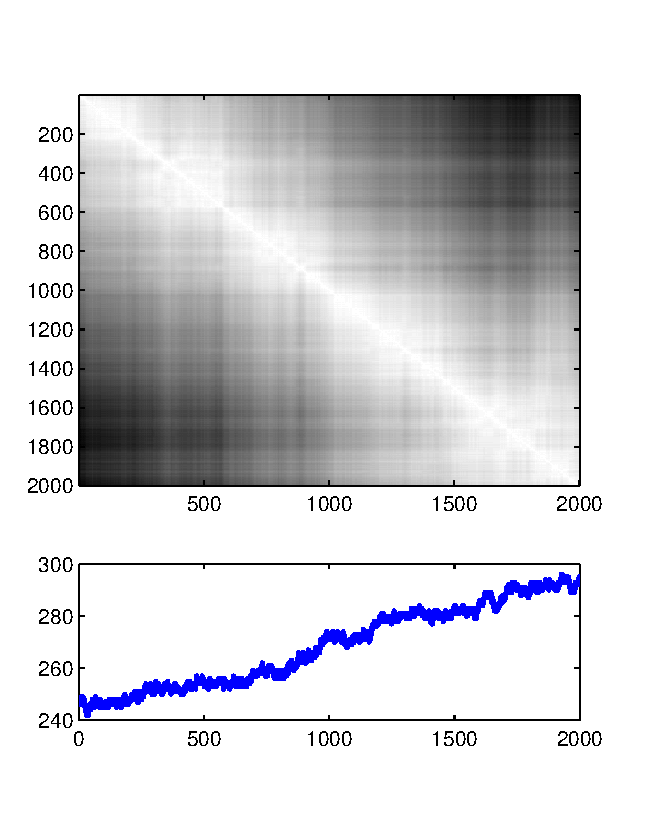
\includegraphics[width=0.9\linewidth]{RW_maps_pTransition_1.eps}
    \hfill
    \caption{Map of hamming distances between classifiers (top chart)
        and error profile (bottom chart) produced by a~simple random walk}
    \label{fig:rwMappingSimple}
    \hfill
    \includegraphics[width=0.9\linewidth]{RW_maps_pTransition_05.eps}
    \hfill
    \caption{Map of hamming distances between classifiers (top chart)
        and error profile (bottom chart) produced by random walk where a step to
        upper vertex is made with probability $0.5$}
    \label{fig:rwMappingPTransition}
\end{multicols}
\end{figure}

To explain the necessity of the parameter~$p$
we presents the results of the simplest random walk with~$n = 2000$ iterations
on fig.~\ref{fig:rwMappingSimple}.
The bottom chart displays the number of errors $n(v_i, \XX)$ as a function of step.
The upper chart displays a color map of pairwise hamming distances $\rho(v_i, v_j)$
between sampled vertices~$v_i$ and~$v_j$.
As a starting point we used a classifier learned by logistic regression.
It is natural to expect that it has relatively small number of errors which drifts upwards along random walk.
This effect is undesired, because classifiers with high number of errors have too small chance to be selected by learning algorithm.

Fig. \ref{fig:rwMappingPTransition} presents similar result for updated random walk
where a step to upper vertex is made with probability $p = 0.5$.
This enforces random walk to stay within the lower layers of the graph.

\section{Experiment}
\label{sec:Experiment}

The goal of our experiment on the benchmark datasets is twofold.
First, we check whether combinatorial functionals
$Q_\eps(\mu,\XX)$ \eqref{eq:QEps} and
$\bar\nu_\ell(\mu,\XX)$ \eqref{eq:avgTestNu}
together with algorithm \ref{alg:walking}
provide an accurate estimates of the overfitting on the hold-out testing sample.
Second, we compare direct Monte-Carlo estimates of overfitting based on functional \eqref{eq:QEps} with
VC-type bound \eqref{eq:VCbound}, SC-bound \eqref{eq:SC-bound},
and with recent PAC-bayesian DD-margin and DI-margin bounds proposed in~\cite{jin2012pacbayes}.

\begin{table}[h]
\caption{Description of datasets}
\label{tab:datasets}
    \centering
    \begin{tabular}[t]{||c|c|c||c|c|c||}
    \hline
    Dataset&\#Examples&\#Features&Dataset&\#Examples&\#Features \\
\hline
    Sonar      & 208   & 60 &    Glass      & 214     &  9 \\
    Liver dis. & 345   &  6 &    Ionosphere & 351     & 34 \\
    Wdbc       & 569   & 30 &    Australian & 690     &  6 \\
    Pima       & 768   &  8 &    Faults     & 1941    & 27 \\
    Statlog    & 2310  & 19 &    Wine       & 4898    & 11 \\
    Waveform   & 5000  & 21 &    Pageblocks & 5473    & 10 \\
    Optdigits  & 5620  & 64 &    Pendigits  & 10992   & 16 \\
    Letter     & 20000 & 16 &               &         &    \\
\hline
\end{tabular}
\end{table}

We use 15 datasets from the UCI repository~\cite{blake98uci}.
If the dataset is a multiclass problem, we manually group the data into two classes since we study binary classification problem.
For preprocessing we eliminate objects with one or more missing features and normalize all features into $[0, 1]$ interval.
A~description of the datasets is given in Table~\ref{tab:datasets} with number of examples after elimination.

In all experiments we split the original dataset $\XX$ into a training sample $\XX_L$ and a testing sample~$\XX_K$.
The training sample $\XX_L$ is used to train a logistic regression and calculate overfitting bounds.
Then we compare predictions of the bounds with the actual error rate on $\XX_K$.

\begin{figure}[t]
    \begin{tabular}{ccc}
        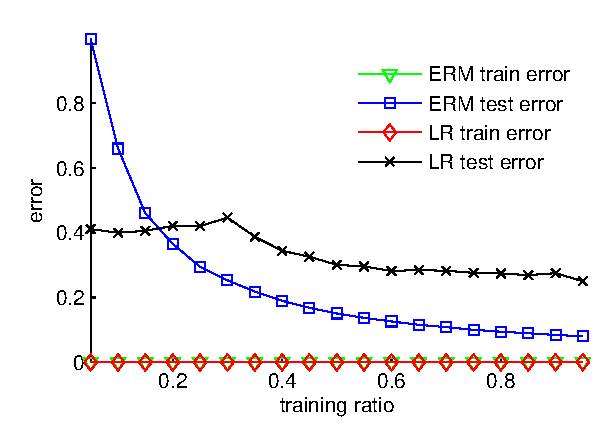
\includegraphics[width=44mm,height=30mm]{Sonar.eps} &
        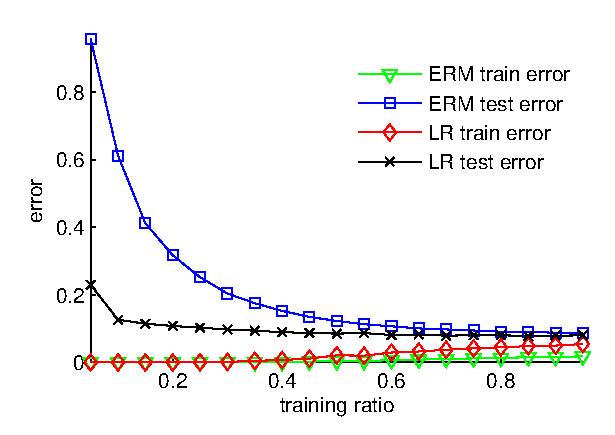
\includegraphics[width=44mm,height=30mm]{glass.eps} &
        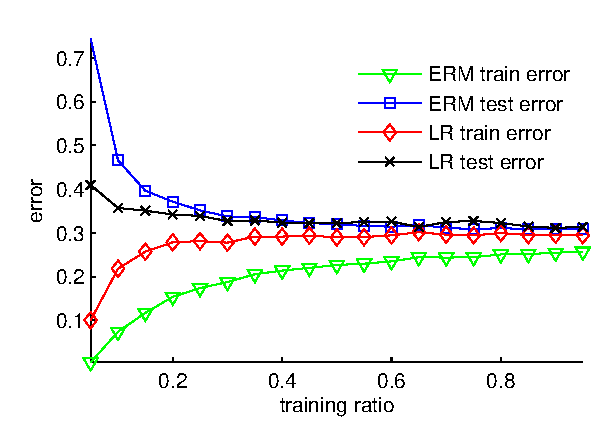
\includegraphics[width=44mm,height=30mm]{Liver_Disorders.eps} \\
        Sonar &
        glass &
        Liver Dis. \\
        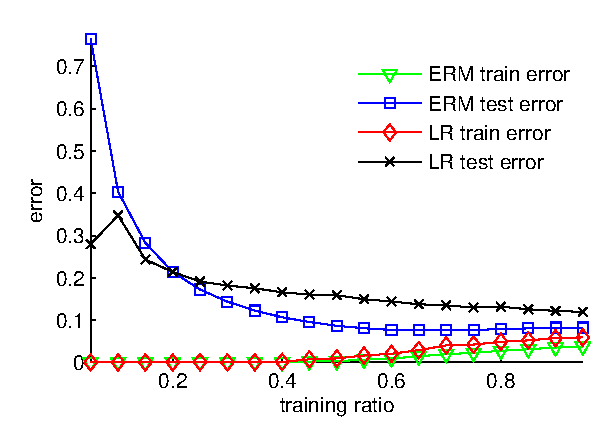
\includegraphics[width=44mm,height=30mm]{Ionosphere.eps} &
        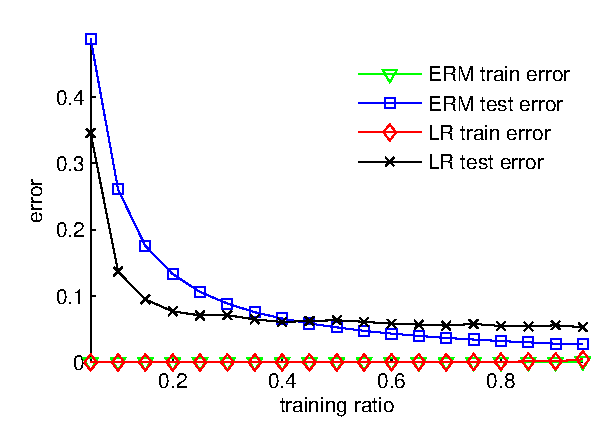
\includegraphics[width=44mm,height=30mm]{Wdbc.eps} &
        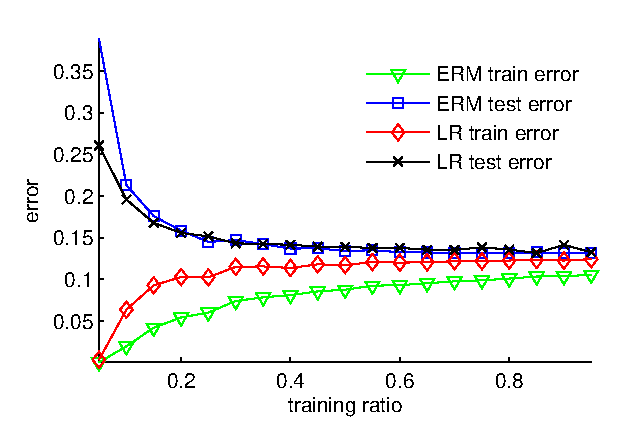
\includegraphics[width=44mm,height=30mm]{Australian.eps} \\
        Ionosphere &
        Wdbc &
        Australian \\
        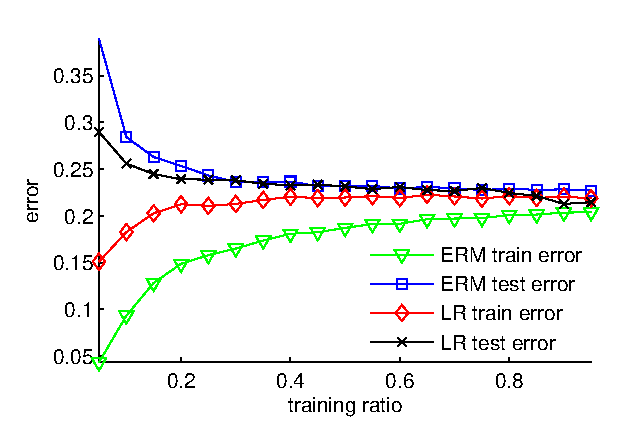
\includegraphics[width=44mm,height=30mm]{pima.eps} &
        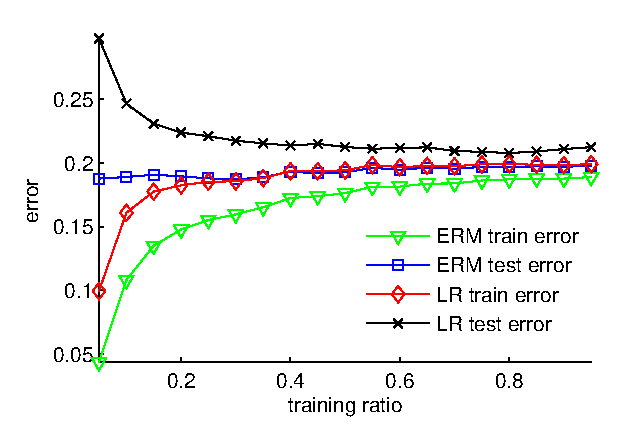
\includegraphics[width=44mm,height=30mm]{faults.eps} &
        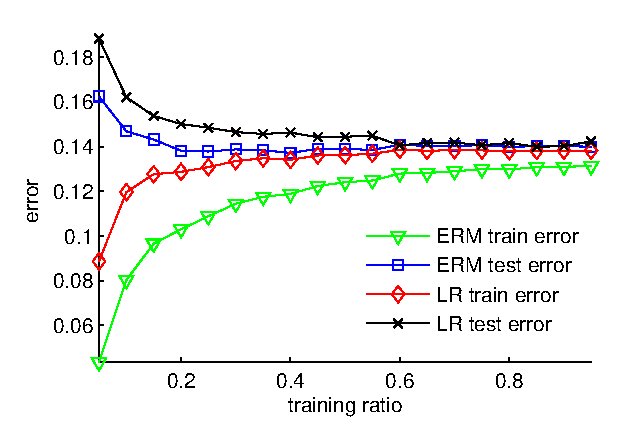
\includegraphics[width=44mm,height=30mm]{statlog.eps} \\
        pima &
        faults &
        statlog \\
        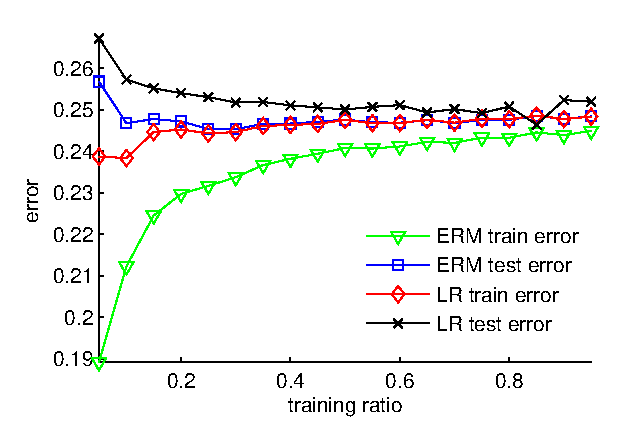
\includegraphics[width=44mm,height=30mm]{wine.eps} &
        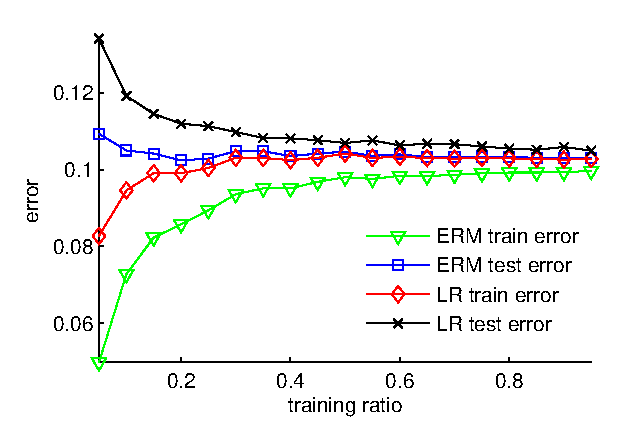
\includegraphics[width=44mm,height=30mm]{waveform.eps} &
        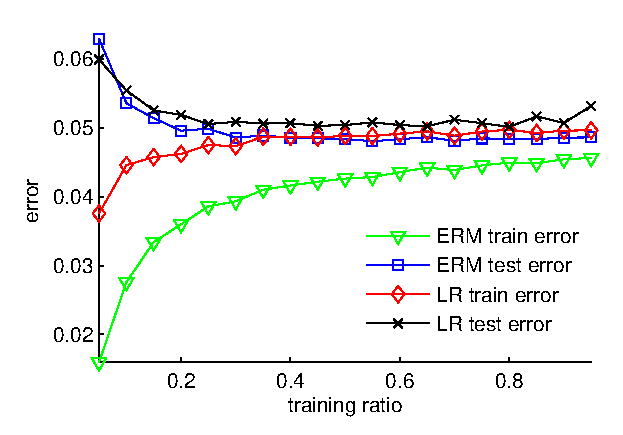
\includegraphics[width=44mm,height=30mm]{pageblocks.eps} \\
        wine &
        waveform &
        pageblocks \\
        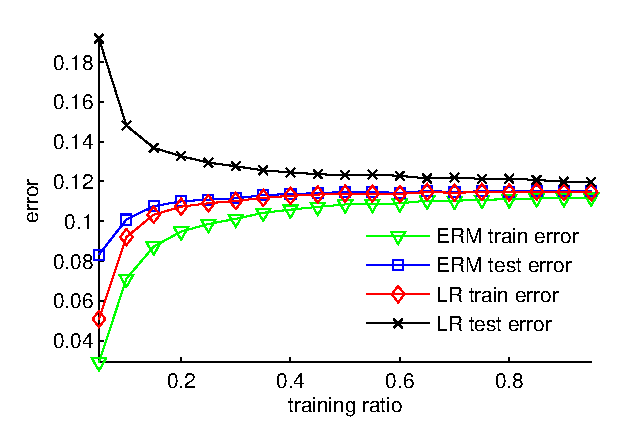
\includegraphics[width=44mm,height=30mm]{Optdigits.eps} &
        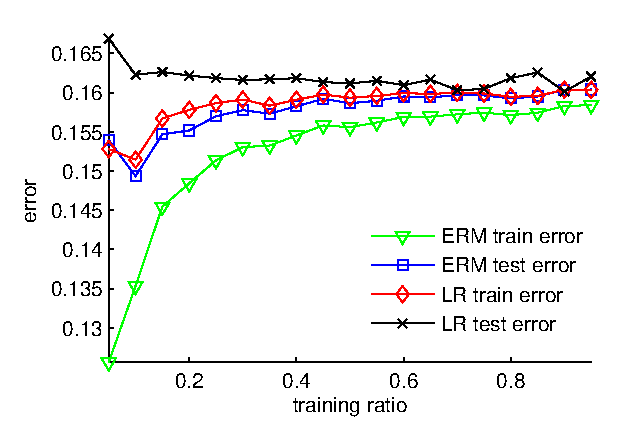
\includegraphics[width=44mm,height=30mm]{pendigits.eps} &
        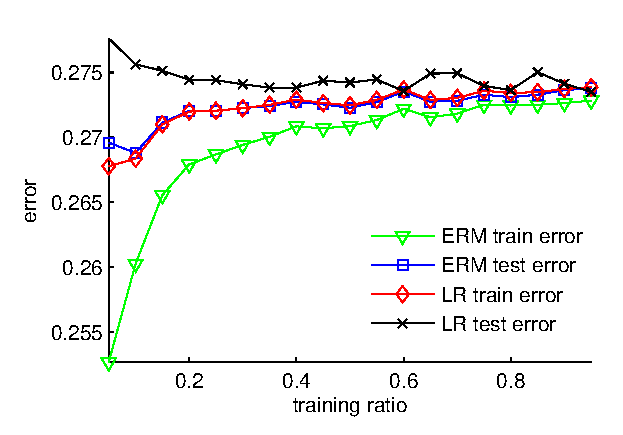
\includegraphics[width=44mm,height=30mm]{Letter.eps} \\
        Optdigits &
        pendigits &
        Letter \\
    \end{tabular}
    \caption{Learning curves of logistic regression and ERM.
        The error ratio of logistic regression is estimated by Monte-Carlo method on splits
        of the original dataset~$\XX = \XX_L \cup \XX_K$.
        The error ratio of ERM is estimated on splits of the training set~$\XX_L = X_\ell \cup X_k$.}
    \label{fig:LearningCurves}
\end{figure}


In the first experiment we build learning curves of logistic regression,
where $L$ runs from 5\% to 95\% of the original dataset size with 5\% steps.
For each~$L$ we generate~$M = 100$ splits ${\XX = \XX_L^i \cup \XX_K^i}$,\; ${i = 1, \dots, M}$
and use them to get Monte-Carlo estimates
of train error rate~$\nu_L(\mu_\LR, \XX)$ from~\eqref{eq:avgTrainNu}
and test error rate~$\bar \nu_L(\mu_\LR, \XX)$ from~\eqref{eq:avgTestNu}
for logistic regression learning algorithm~$\mu_\LR$:
\[
    \hat \nu_L(\mu_\LR, \XX)
    =
    \frac{1}{M} \sum_{i = 1}^{M} \nu(\mu_\LR \XX_L^i, \XX_L^i),
    \qquad
    \hat{\bar \nu}_L(\mu_\LR, \XX)
    =
    \frac{1}{M} \sum_{i = 1}^{M} \nu(\mu_\LR \XX_L^i, \XX_K^i).
\]

After that for each training sample~$\XX_L$ we sample classifiers
and estimate an average ERM errors:
train error $\nu_\ell(\mu, \XX_L)$
and test error $\bar \nu_\ell(\mu, \XX_L)$,
where $\mu$ is ERM learning algorithm.
To sample classifiers on $\XX_L$ we launch algorithm \ref{alg:walking}
with parameters $n=8\,192$, $N = 64$, $m = 15$, $p = 0.8$,
and use classifier~$\mu_\LR \XX_L$ as a starting point.
To estimate $\nu_\ell(\mu, \XX_L)$ and $\bar \nu_\ell(\mu, \XX_L)$ we again compute Monte-Carlo type
estimates of definitions \eqref{eq:avgTrainNu} and \eqref{eq:avgTestNu}
by randomly generating $M' = 4\,096$ splits $\XX_L = X_\ell^j \cup X_k^j$,
$j = 1, \dots, M'$, at constant ratio $\frac{\ell}{L} = 0.8$:
\[
    \hat \nu_\ell(\mu, \XX_L)
    =
    \frac{1}{M'} \sum_{j = 1}^{M} \nu(\mu X_\ell^j, X_\ell^j),
    \qquad
    \hat{\bar \nu}_\ell(\mu, \XX_L)
    =
    \frac{1}{M'} \sum_{j = 1}^{M} \nu(\mu X_\ell^j, X_k^j).
\]
These estimates are then averaged over all partitions~$\XX = \XX_L^i \cup \XX_K^i$.

The four values (the actual train and test errors of logistic regression
$\nu_L(\mu_\LR, \XX)$ and $\bar \nu_L(\mu_\LR, \XX)$,
ERM train error $\nu_\ell(\mu, \XX_L)$, and ERM test error $\bar \nu_\ell(\mu, \XX_L)$)
are charted as a functions of a training sample size ratio, see Figure \ref{fig:LearningCurves},
sorted according to sizes of datasets, from the smallest to the largest.
Note that ERM test error might be either below or above
actual test error rate of logistic regression
because~$\mu$ and~$\mu_\LR$ are quite different learning algorithms.
However, from charts we conclude that $\bar \nu_\ell(\mu, \XX_L)$,
estimated only based on $\XX_L$, provides reasonably good estimate
of actual test error rate $\bar \nu_L(\mu_\LR, \XX)$
and of the learning curve on test sample $\XX_K$.

Now we turn to comparison of different overfitting bounds.
For each dataset we use 5-fold cross validation and average the results over 20 runs (for a total 100 runs).
As before, we use training sample~$\XX_L$ to learn logistic regression,
run algorithm \ref{alg:walking}, and
estimate $\nu_\ell(\mu, \XX_L)$ and $\bar \nu_\ell(\mu, \XX_L)$
based on $4\,096$ randomly generated splits $\XX_L = X_\ell^j \cup X_k^j$.
In addition, we use $\XX_L$ to estimate overfitting
$\bar \nu_\ell(\mu, \XX_L) - \nu_\ell(\mu, \XX_L)$
by medians of VC-type bound \eqref{eq:VCbound} and SC-bound \eqref{eq:SC-bound},
and to calculate DD-margin and DI-margin bounds from~\cite{jin2012pacbayes}.
The results are presented in Table \ref{tab:compareToPacBayes}.
Note that while all combinatorial bounds estimate overfitting, PAC DI and PAC DD are upper bounds on the test error.

Our key observation is that $\delta_\ell(\mu) \equiv \bar \nu_\ell(\mu, \XX_L) - \nu_\ell(\mu, \XX_L)$
is in the order of magnitude sharper than any of the other bounds.
It works well for all datasets except Sonar~(which is the smallest dataset in our selection).
Across combinatorial bounds the SC-bound outperform VC-type bound, but still vastly overestimates the target quantity $\delta_\ell(\mu)$.
All combinatorial bounds provide tighter estimates on overfitting and test error rate than PAC-Bayesian bounds.

Note that the VC-bound is estimated by a small subset of~$A$ obtained from a~random walk.
This is a~``localized'' VC-bound.
The usual VC-bound estimated from VC-dimension~$d$ of a~whole set~$A$ should be greater than~1 on all datasets.

\begin{table}[t]
      \caption{Comparison between real overfitting and various overfitting bounds.
        TrainErr stands for $\nu_L(\mu_\LR, \XX)$,
        TestErr for $\bar \nu_L(\mu_\LR, \XX)$,
        Overfit is their difference, %for $\bar \nu_L(\mu_\LR, \XX) - \nu_L(\mu_\LR, \XX)$
        $\delta_\ell(\mu) \equiv \bar \nu_\ell(\mu, \XX_L) - \nu_\ell(\mu, \XX_L)$.}
      \label{tab:compareToPacBayes}
      \centering
        \begin{tabular}[t]{||l||r|r|r||r|r|r|r|r|r||}
        \hline
        &
        \multicolumn{4}{|c|}{Monte-Carlo estimates}&
        \multicolumn{4}{|c|}{Generalization bounds} \\
        \hline
            Task&
            TrainErr &
            TestErr &
            Overfit &
            $\delta_\ell(\mu)$&
            VC&
            SC&
            PAC DI&
            PAC DD \\
        \hline
            Sonar       & 0.000 & 0.271 & 0.271 & 0.095 & 0.185 & 0.119 & 1.287 & 1.287 \\
            glass       & 0.046 & 0.075 & 0.029 & 0.078 & 0.211 & 0.140 & 1.126 & 0.738 \\
            Liver dis.  & 0.299 & 0.314 & 0.015 & 0.060 & 0.261 & 0.209 & 1.207 & 1.067 \\
            Ionosphere  & 0.049 & 0.125 & 0.077 & 0.052 & 0.150 & 0.112 & 1.219 & 1.153 \\
            Wdbc        & 0.001 & 0.056 & 0.055 & 0.032 & 0.071 & 0.043 & 1.174 & 0.705 \\
            Australian  & 0.122 & 0.136 & 0.013 & 0.030 & 0.137 & 0.110 & 1.146 & 0.678 \\
            pima        & 0.220 & 0.227 & 0.007 & 0.028 & 0.159 & 0.127 & 0.971 & 0.749 \\
            faults      & 0.198 & 0.210 & 0.012 & 0.010 & 0.108 & 0.087 & 1.110 & 1.061 \\
            statlog     & 0.138 & 0.142 & 0.005 & 0.010 & 0.096 & 0.082 & 1.102 & 0.747 \\
            wine        & 0.248 & 0.250 & 0.002 & 0.004 & 0.134 & 0.109 & 0.776 & 0.637 \\
            waveform    & 0.103 & 0.105 & 0.002 & 0.004 & 0.099 & 0.079 & 0.561 & 0.354 \\
            pageblocks  & 0.050 & 0.050 & 0.001 & 0.004 & 0.073 & 0.057 & 0.737 & 0.186 \\
            Optdigits   & 0.115 & 0.121 & 0.006 & 0.004 & 0.102 & 0.084 & 1.068 & 0.604 \\
            pendigits   & 0.160 & 0.161 & 0.001 & 0.002 & 0.127 & 0.103 & 0.774 & 0.432 \\
            Letter      & 0.274 & 0.274 & 0.001 & 0.001 & 0.165 & 0.137 & 0.818 & 0.636 \\
        \hline
        \end{tabular}
    \end{table}

\section{Conclusion}
In this paper we present a new random walk based technique for efficient calculation of
combinatorial data-dependent generalization bounds.
Although combinatorial bounds are obtained for empirical risk minimization under binary loss,
we~show that they provide sharp overfitting estimates for logistic regression.
Our~bounds
recover a correct shape of the learning curves of logistic regression,
correlates well with its actual overfitting,
and outperform  both classical VC-bound and recent state-of-the-art PAC-Bayesian bounds
in~experiments on 15~datasets from the UCI repository.

%\small{
\begin{thebibliography}{00}
\bibitem{agarwal98arrangements}
    Agarwal\;P.\,K., Sharir\;P.~(1998)
    Arrangements and their applications~//
    In \emph{Handbook of Computational Geometry}, 49--119.

\bibitem{blake98uci}
    Asuncion\;A, Newman\;D.\,J.~(2007)
    UCI Machine Learning Repository.
    \emph{University of California, Irvine, School of Information and Computer Sciences}

\bibitem{avrachenkov10restarts}
    Avrachenkov\;K., Ribeiro\;B., Towsley\;D.~(2010)
    Improving random walk estimation accuracy with uniform restarts.
    {\it Proc. of WAW 2010}.

\bibitem{bax97similar}
    Bax\;E.~(1997)
    Similar classifiers and VC error bounds.

\bibitem{boucheron05survey}
     Boucheron\;S., Bousquet\;O., Lugosi\;G.~(2005)
     Theory of classification: A survey of some recent advances.
     \emph{ESAIM: probability and statistics}, 9(1), 323--375.

\bibitem{haussler94predicting}
     Haussler\;D., Littlestone\;N., Warmuth\;M.\,K.~(1994)
     Predicting $\{0, 1\}$-functions on randomly drawn points.
     \emph{Information and Computation}, 115(2), 248--292.

\bibitem{jin2012pacbayes}
     Jin\;C., Wang\;L.~(2012)
     Dimensionality Dependent PAC-Bayes Margin Bound.
     \emph{In Advances in Neural Information Processing Systems}, 25, 1043--1051.

\bibitem{koltchinskii06rademacher}
     Koltchinskii\;V.~(2006)
     Local Rademacher complexities and oracle inequalities in risk minimization (with discussion).
     \emph{The Annals of Statistics}, 34, 2593-2706.

\bibitem{koltchinskii02margin}
    Koltchinskii\;V., Panchenko\;D.~(2002)
    Empirical margin distributions and bounding the generalization error of combined classifiers.
    \emph{The Annals of Statistics}, 30(1), 1-50.

\bibitem{koltchinskii03convex}
    Koltchinskii\;V., Panchenko\;D.~(2003)
    Bounding the generalization error of convex combinations of classifiers: balancing the dimensionality and the margins.
    \emph{The Annals of Applied Probability}, 13(1), 213-252.

\bibitem{lee12backtrack}
    Lee\;C., Xu\;X., Eun\;D.~(2012)
    Beyond Random Walk and Metropolis-Hastings Samplers: Why You Should Not Backtrack for Unbiased Graph Sampling.
    \emph{ACM SIGMETRICS Performance Evaluation Review}, 40(1), 319--330.

\bibitem{lugosi03concentration}
     Lugosi\;G.~(2003)
     On concentration-of-measure inequalities.
     \emph{Machine Learning Summer School}, Australian National University, Canberra.

\bibitem{ribeiro10multidimensional}
    Ribeiro\;B., Towsley\;D.~(2010).
    Estimating and sampling graphs with multidimensional random walks.
    \emph{10th Conf. on Internet Measurement}, 390--403.

\bibitem{vapnik71convergence}
     Vapnik\;V.\,N., Chervonenkis\;A.\,Y.~(1971)
     On the uniform convergence of relative frequencies of events to their probabilities.
     \emph{Theory of Probability and Its Applications}, 16(2), 264--280.

\bibitem{voron09overfitting}
    Vorontsov\;K.\,V.~(2009)
    Splitting and similarity phenomena in the sets of classifiers and their effect on the probability of overfitting.
    \emph{Pattern Recognition and Image Analysis}, 19(3), 412--420.

\bibitem{voron11premi}
    Vorontsov\;K.\,V., Ivahnenko\;A.\,A.~(2011)
    Tight combinatorial generalization bounds for threshold conjunction rules.
    \emph{4-th Int'l Conf. on Pattern Recognition and Machine Intelligence (PReMI'11)}.
    Lecture Notes in Computer Science, Springer-Verlag, 66--73.

\end{thebibliography}
%}

%%%\newpage
%%%\section*{Appendix}
%%%\newcommand{\wtil}{\widetilde}
%%%\def\XYtext(#1,#2)#3{\rlap{\kern#1\lower-#2\hbox{#3}}}
%%%
%%%
%%%\begin{theorem}[FC-bound]
%%%\label{thOneAlg}
%%%    For any set $\XX$,
%%%    any $\eps\in [0,1]$,
%%%    and a~fixed classifier~$a$ such that ${m=n(a,\XX)}$
%%%    the probability of~overfitting is~given by the left tail of the hypergeometric distribution:
%%%    \begin{equation}
%%%    \label{eq:OCbound}
%%%        Q_\eps(a, \XX)
%%%        %\Prbig[ \delta(a,X) \geq \eps ]
%%%        =
%%%        \Hyper{L}{m}{\ell}{ \tfrac{\ell}{L} (m-\eps k) }.
%%%    \end{equation}
%%%\end{theorem}
%%%\begin{proof}
%%%    Denote ${s=n(a,X)}$ and rewrite the overfitting condition
%%%    ${\delta(a,X) \geq \eps}$
%%%    as
%%%    $\tfrac1k (m-s) - \tfrac{1}{\ell} s \geq \eps$
%%%    or equivalently
%%%    ${s \leq \tfrac{\ell}{L} (m-\eps k) \eqdef s_m(\eps) }$. Then
%%%    \[
%%%        Q_\eps
%%%        =
%%%        \Prob\bigl[
%%%            n(a,X) \!\leq\! s_m(\eps)
%%%        \bigr]
%%%        =
%%%        \sum\limits_{s=s_0}^{\lfloor s_m(\eps) \rfloor}
%%%        \Prob\bigl[
%%%            n(a,X) \!=\! s
%%%        \bigr]
%%%        =
%%%        \sum\limits_{s=s_0}^{\lfloor s_m(\eps) \rfloor}
%%%        \hyper{L}{m}{\ell}{s}
%%%        =
%%%        \Hyper{L}{m}{\ell}{ s_m(\eps) }.
%%%    \]
%%%    \vskip-3ex
%%%\end{proof}
%%%
%%%\begin{theorem}[VC-bound]
%%%\label{thOneAlg}
%%%    For any set $\XX$,
%%%    any learning algorithm~$\mu$,
%%%    and any $\eps\in [0,1]$
%%%    the probability of~large uniform deviation is bounded by the sum of FC-bounds over the set~$A$:
%%%    \begin{equation}
%%%    \label{eq:VCbound}
%%%        %Q_\eps(\mu, \XX)
%%%        \wtil Q_\eps(A, \XX)
%%%        %\Prbig[ \delta(a,X) \geq \eps ]
%%%        \leq
%%%        \sum_{a\in A}
%%%        \Hyper{L}{m}{\ell}{ \tfrac{\ell}{L} (m-\eps k) },
%%%        \quad
%%%        m = n(a,\XX).
%%%    \end{equation}
%%%\end{theorem}
%%%\begin{proof}
%%%    %Apply a union bound which is in fact a substitute of binary values sum for their maximum:
%%%     Apply a union bound substituting the maximum of binary values by their sum:
%%%    \[
%%%        \wtil Q_{\eps} =
%%%        \Prob
%%%        \max_{a\in A}
%%%        \bigl[
%%%            \delta(a,X) \!\geq\! \eps
%%%        \bigr]
%%%        \leq
%%%        \sum_{a\in A}
%%%        \Prob
%%%        \bigl[
%%%            \delta(a,X) \!\geq\! \eps
%%%        \bigr]
%%%        =
%%%        \sum_{a\in A}
%%%        \Hyper{L}{m}{\ell}{s_m(\eps)},
%%%        \quad
%%%        m = n(a).
%%%    \]
%%%    \vskip-3ex
%%%\end{proof}
%%%
%%%Further weakening gives a~well known form of the VC-bound:
%%%\[
%%%    \wtil Q_\eps(A, \XX)
%%%    \leq
%%%    |A| \max_m \Hyper{L}{m}{\ell}{s_m(\eps)}
%%%    \leq
%%%    |A| \cdot \tfrac32 e^{-\eps^2\ell},
%%%    \quad
%%%    \text{if } \ell=k,
%%%\]
%%%where $|A|$ is~called a \emph{shattering coefficient} of~the set of classifiers~$A$ on~the~set~$\XX$.
%%%
%%%\subsection*{The principle of protective and prohibitive subsets}
%%%\label{sec:ProtProh}
%%%
%%%The principle of protective and prohibitive sets~\cite{voron10pria-eng}
%%%is based on the conjecture that
%%%the necessary and sufficient condition for $\mu X=a$ can be specified explicitly
%%%for any classifier $a\in A$
%%%in~terms of subsets of~objects.
%%%From this conjecture an exact $Q_\eps$ bound has been derived.
%%%
%%%In~this work we use a similar conjecture relaxed to the necessary condition
%%%and derive an upper bound which has a~simpler form.
%%%
%%%\begin{theorem}
%%%\label{hyp:1}
%%%    For each classifier $a\in A$  there exists
%%%    a~\emph{protective subset} $X_a\in \XX$ and
%%%    a~\emph{prohibitive subset} $X'_a\in \XX$ such that
%%%    for any $X\in\XXell$
%%%    \begin{equation}
%%%    \label{eq:hyp1}
%%%    	\bigl[ \mu X \!=\! a \bigr] \leq
%%%        \bigl[X_a \!\subseteq\! X \bigr]
%%%        \bigl[X'_a \!\subseteq\! \X \bigr].
%%%    \end{equation}
%%%\end{theorem}
%%%
%%%The subset $\XX{\setminus} X_a{\setminus} X'_a$
%%%is~called \emph{neutral} for a~classifier~$a$.
%%%The presence or absence of neutral objects in a~training sample~$X$
%%%does not change the result of learning~$\mu X$.
%%%Later we will give nontrivial examples of $\mu$ and $A$ that satisfy conjecture~\ref{hyp:1}.
%%%
%%%\begin{lemma}
%%%\label{lem1}
%%%    If conjecture~\ref{hyp:1} holds,
%%%    then the probability to~learn a~classifier~$a$ can be bounded:
%%%    \[
%%%        \Prbig[ \mu X\!=\!a ]
%%%        \leq
%%%        P_a
%%%        \equiv
%%%        {\CC_{L_a}^{\ell_a}} / {\CC_{L}^{\ell}},
%%%    \]
%%%    where
%%%    $L_a = L - |X_a| - |X'_a|$ and
%%%    $\ell_a = \ell - |X_a|$
%%%    are the number of neutral objects for~a~classifier~$a$ in the general set~$\XX$ and sample~$X$ respectively.
%%%\end{lemma}
%%%\begin{proof}
%%%    According to the conjecture
%%%    ${
%%%        \Prbig[ \mu X\!=\!a ]
%%%        \leq
%%%        \Prob
%%%        \bigl[  X_a\subseteq  X \bigr]
%%%        \bigl[ X'_a\subseteq \X \bigr]
%%%    }$.
%%%    The right-hand side
%%%    is a fraction of~partitions ${\XX=X\sqcup\X}$ such that
%%%    ${X_a\subseteq  X}$ and ${X'_a\subseteq  \X}$.
%%%    The number of~such partitions is equal to~$\CC_{L_a}^{\ell_a}$.
%%%    The number of all partitions is equal to~$\CC_{L}^{\ell}$,
%%%    hence their ratio gives~$P_a$.
%%%\end{proof}
%%%
%%%\begin{theorem}
%%%\label{th:1}
%%%    If conjecture~\ref{hyp:1} holds, then
%%%    for any $\eps\in[0,1]$
%%%    the bound on probability of overfitting is
%%%    \begin{equation}
%%%    \label{eq:th1}
%%%        Q_\eps
%%%        \leq
%%%        \sum_{a\in \AA} P_a \Hyper{L_a}{m_a}{\ell_a}{s_a(\eps)},
%%%    \end{equation}
%%%    where
%%%    ${m_a = n(a,\XX{\setminus} X_a {\setminus} X'_a)}$
%%%    is a~number of errors that classifier~$a$ produces on~neutral objects and
%%%    ${s_a(\eps) = \tfrac\ell L \bigl( n(a)-\eps k \bigr) - n(a,X_a)}$
%%%    is a~largest number of errors $n(a,X{\setminus}X_a)$
%%%    that classifier~$a$ produces on~neutral training objects
%%%    provided that discrepancy $\delta(a,X)$ exceeds~$\eps$.
%%%\end{theorem}
%%%
%%%\begin{proof}
%%%    The probability of~overfitting~$Q_\eps$
%%%    can be found as a total probability
%%%    from probability to~learn each of classifiers $\Prbig[ \mu X\!=\!a ]$
%%%    and conditional probabilities
%%%    ${
%%%        Q_{\eps|a} = \Prbig[ \delta(a,X) \!\geq\! \eps \mid a\!=\!\mu X ]
%%%    }$:
%%%    \[
%%%        Q_\eps
%%%        =
%%%        \sum_{a\in \AA}
%%%            \Prbig[ \mu X\!=\!a ] Q_{\eps|a}
%%%        \leq
%%%        \sum_{a\in \AA}
%%%            P_a Q_{\eps|a}.
%%%    \]
%%%    The conditional probability $Q_{\eps|a}$ can be obtained from theorem~\ref{thOneAlg}
%%%    by~taking into account that
%%%    the subsets $X_a$ and $X'_a$ can not be involved in~partitioning given a~fixed classifier~$a$.
%%%    Only $L_a$~neutral objects are partitioned
%%%    into $\ell_a$~training and $L_a-\ell_a$ testing objects.
%%%    To~employ theorem~\ref{thOneAlg} we~express the discrepancy $\delta(a,X)$
%%%    in~terms or the number of errors on neutral training objects $s = n(a,X{\setminus} X_a)$:
%%%    \[
%%%        \delta(a,X) =
%%%        \tfrac1k \bigl( n(a)-s-n(a,X_a) \bigr) -
%%%        \tfrac1\ell \bigl( s+n(a,X_a) \bigr).
%%%    \]
%%%    Condition $\delta(a,X)\geq \eps$ is~equivalent to $s\leq s_a(\eps)$.
%%%    Then $Q_{\eps|a} = \Hyper{L_a}{m_a}{\ell_a}{ s_a(\eps) }$
%%%    and~\eqref{eq:th1} holds.
%%%\end{proof}
%%%
%%%Note that the sum $\sum_a P_a$ can be interpreted
%%%as a~degree of looseness of the bound~\eqref{eq:th1}.
%%%The~bound is~exact if this sum is equal to~1.
%%%
%%%\medskip
%%%The principle of protective and prohibitive subsets
%%%is a~powerful tool to~obtain combinatorial generalization bounds.
%%%In~\cite{voron10pria-eng} it has been used to obtain exact bounds on probability of overfitting
%%%for model sets of classifiers like monotonic and unimodal chains.
%%%This work is focused on~common bounds for arbitrary sets of classifiers
%%%that take into account both splitting and connectivity properties of~the~set.
%%%
%%%\subsection*{The splitting and connectivity graph}
%%%Define an order relation on classifiers $a\leq b$ as a natural order over their error vectors:
%%%$a_i \leq b_i$ for all $i=1,\ldots,L$.
%%%Define a~metric on classifiers as a Hamming distance between error vectors:
%%%$\rho(a,b) = \sum_{i=1}^L |a_i-b_i|$.
%%%Classifiers $a$ and $b$ are called \emph{connected} if $\rho(a,b) = 1$.
%%%Define the precedence relation on classifiers $a\prec b$ as
%%%$\bigl(a\leq b\bigr) \wedge \bigl( \rho(a,b)=1 \bigr)$.
%%%
%%%%\bigskip
%%%%{\LARGE
%%%%$x_1$ $x_2$ $x_3$ $x_4$ $x_5$ $x_6$ $x_7$ $x_8$ $x_9$ $x_{10}$ }
%%%%\bigskip
%%%
%%%The set of classifiers $A$ can be represented by
%%%a~multipartite directed graph $\langle A, E \rangle$
%%%that we call the \emph{splitting and connectivity graph} (SC-graph)
%%%in which vertices are classifiers, and
%%%edges $(a,b)$ are pairs of classifiers such that $a\prec b$,
%%%see example on~Figure~\ref{fig:SC-graph-lin}.
%%%The partite subsets $A_m = \{ a\in A\colon n(a)=m \}$
%%%are called \emph{error layers}, $m=0,\ldots,L$.
%%%Each edge of the SC-graph $(a,b)$ corresponds to an object $x_{ab}\in\XX$
%%%such that $I(a,x_{ab})=0$ and $I(b,x_{ab})=1$.
%%%
%%%\begin{figure}[t]
%%%    \noindent\centering
%%%    \raisebox{3mm}{(a)~}
%%%    \includegraphics[width = 60mm]{SimpleSample1num.PNG.eps}
%%%    \qquad
%%%    \raisebox{3mm}{(b)~}
%%%    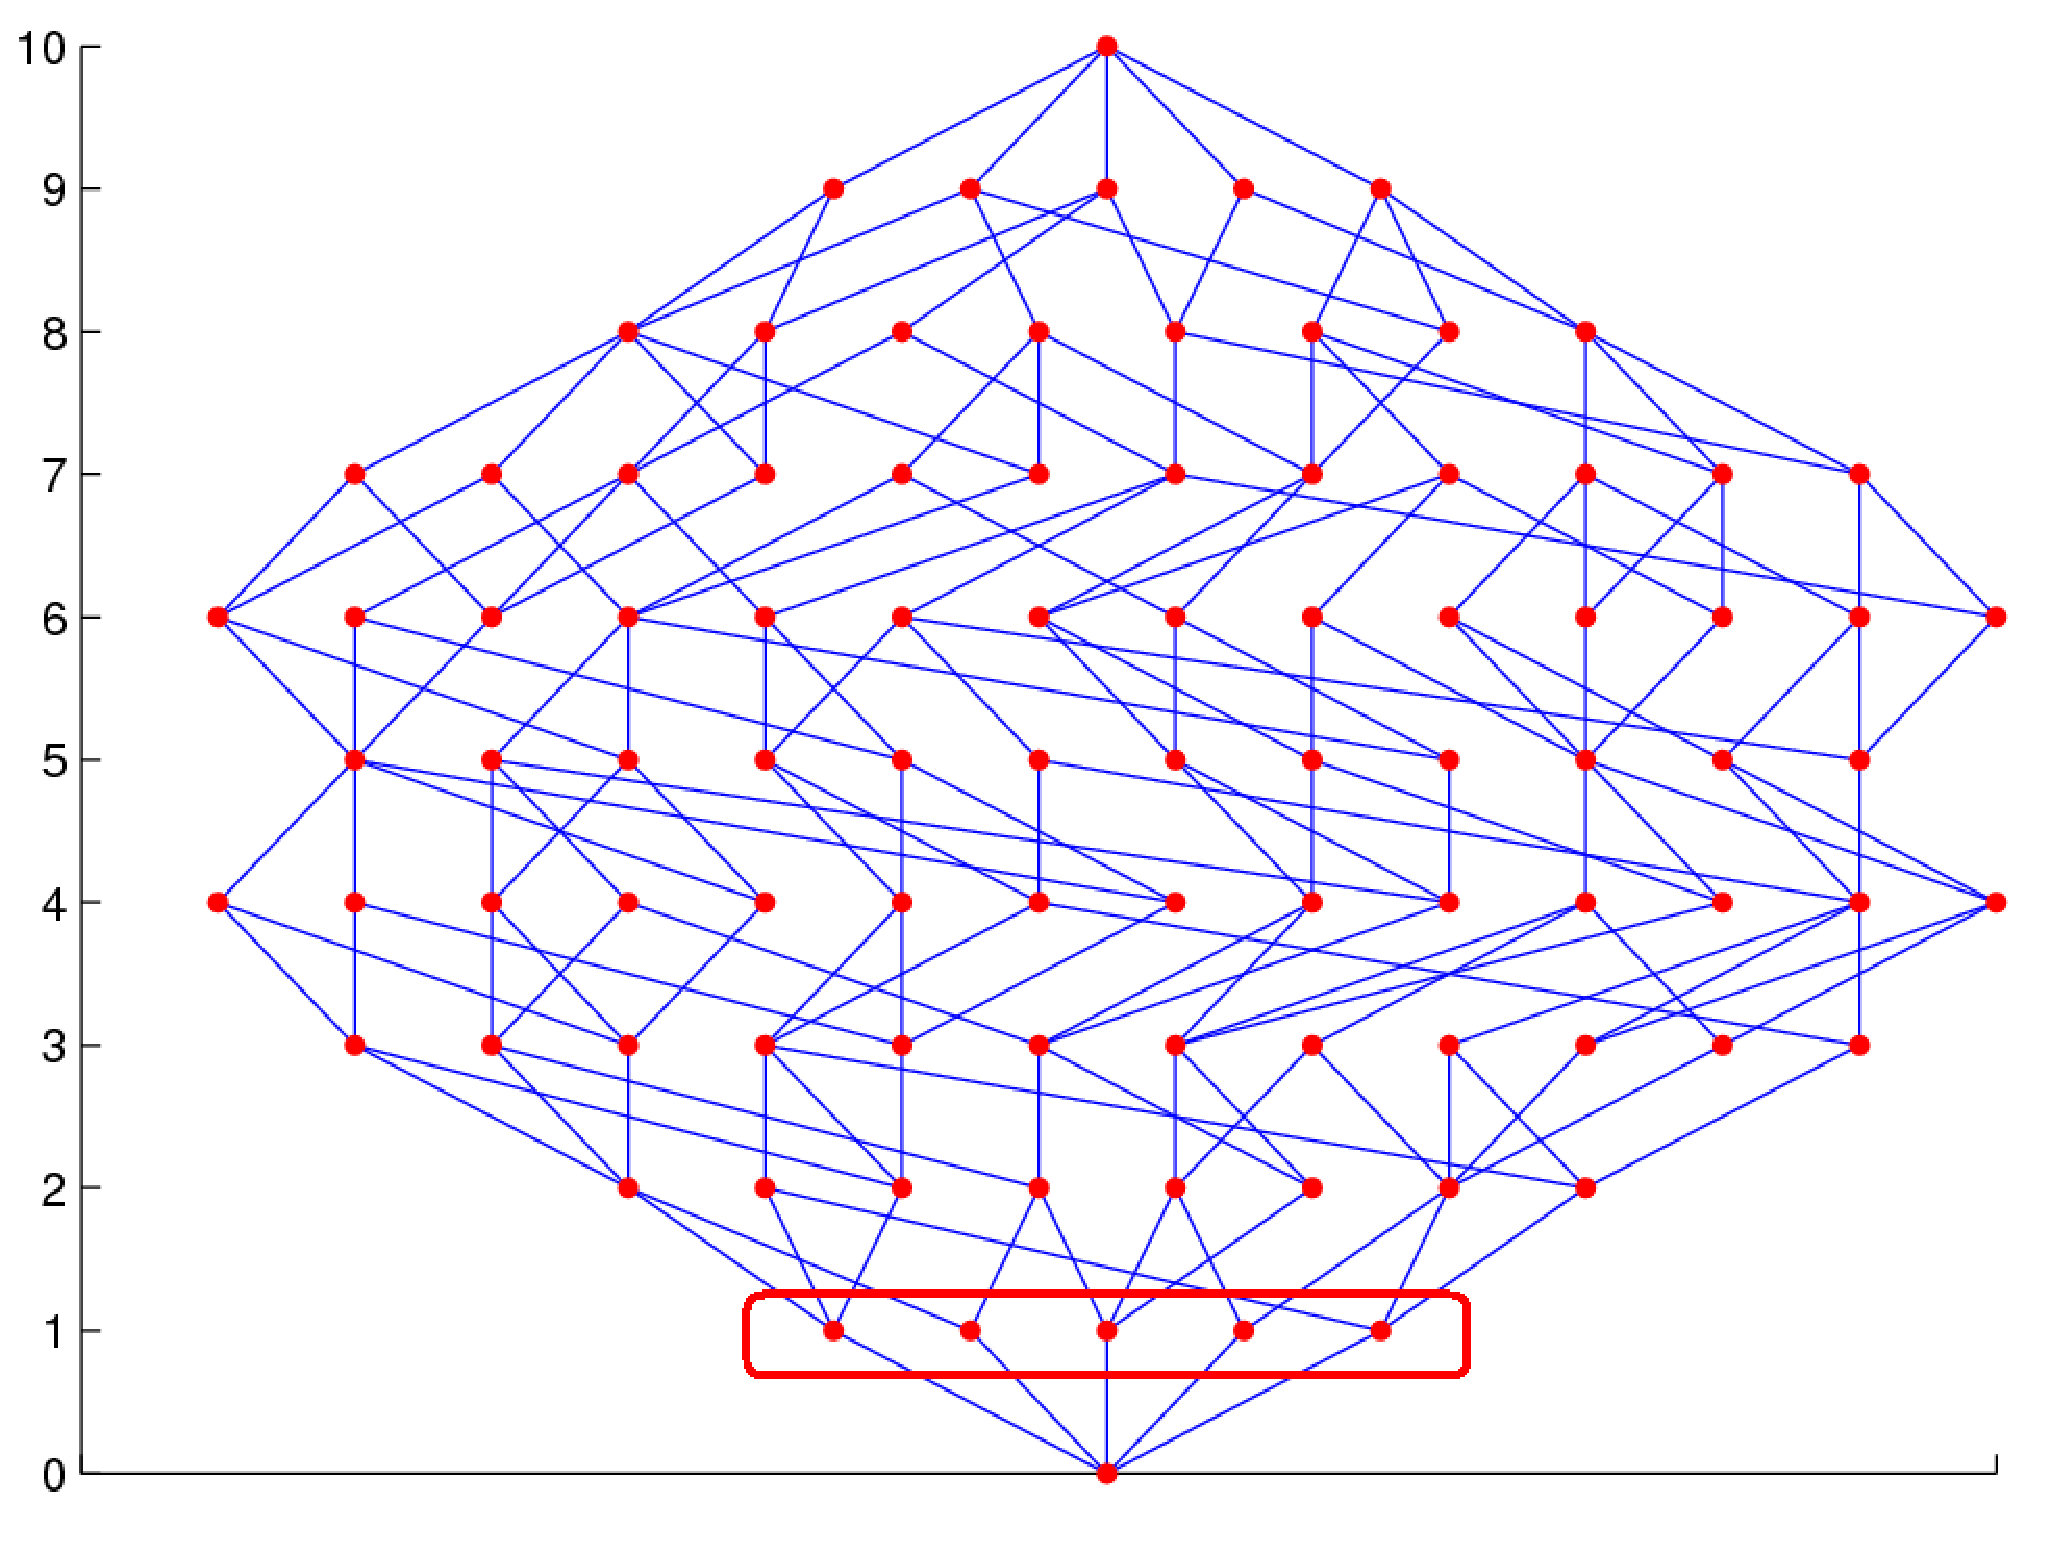
\includegraphics[width = 60mm]{SimpleGraph1.PNG.eps}
%%%    \XYtext(-65mm,43mm){\scriptsize{$m$}}%
%%%    \\\medskip
%%%    \raisebox{-10mm}{(c)}
%%%    \scriptsize
%%%    \begin{tabular}{c|c|ccccc|cccccccc|c}
%%%        & {layer 0} &
%%%        \multicolumn{5}{c|}{layer 1} &
%%%        \multicolumn{8}{c|}{layer 2} \\
%%%        $x_1$ & 0 & 1 & 0 & 0 & 0 & 0 & 1 & 0 & 0 & 0 & 0 & 1 & 1 & 0 & \ldots \\[-0.6ex]
%%%        $x_2$ & 0 & 0 & 1 & 0 & 0 & 0 & 1 & 1 & 0 & 0 & 0 & 0 & 0 & 0 & \ldots \\[-0.6ex]
%%%        $x_3$ & 0 & 0 & 0 & 1 & 0 & 0 & 0 & 1 & 1 & 0 & 0 & 0 & 0 & 1 & \ldots \\[-0.6ex]
%%%        $x_4$ & 0 & 0 & 0 & 0 & 1 & 0 & 0 & 0 & 1 & 1 & 0 & 0 & 0 & 0 & \ldots \\[-0.6ex]
%%%        $x_5$ & 0 & 0 & 0 & 0 & 0 & 1 & 0 & 0 & 0 & 1 & 1 & 1 & 0 & 0 & \ldots \\[-0.6ex]
%%%        $x_6$ & 0 & 0 & 0 & 0 & 0 & 0 & 0 & 0 & 0 & 0 & 1 & 0 & 1 & 0 & \ldots \\[-0.6ex]
%%%        $x_7$ & 0 & 0 & 0 & 0 & 0 & 0 & 0 & 0 & 0 & 0 & 0 & 0 & 0 & 1 & \ldots \\[-0.6ex]
%%%        $x_8$ & 0 & 0 & 0 & 0 & 0 & 0 & 0 & 0 & 0 & 0 & 0 & 0 & 0 & 0 & \ldots \\[-0.6ex]
%%%        $x_9$ & 0 & 0 & 0 & 0 & 0 & 0 & 0 & 0 & 0 & 0 & 0 & 0 & 0 & 0 & \ldots \\[-0.6ex]
%%%     $x_{10}$ & 0 & 0 & 0 & 0 & 0 & 0 & 0 & 0 & 0 & 0 & 0 & 0 & 0 & 0 & \ldots
%%%    \end{tabular}
%%%    \caption{%
%%%        Two-dimensional linearly separable classification task with ${L=10}$ objects of~2~classes
%%%        and 5~linear classifiers that produce exactly one error~(a).
%%%        The~SC-graph over the set of~all \mbox{2-dimensional} linear classifiers~(b).
%%%        The~first layer (${m=1}$) corresponds to 5~classifiers shown at the left chart.
%%%        The~fragment of error matrix corresponding to layers $m=0,1,2$ (c).
%%%    }
%%%    \label{fig:SC-graph-lin}
%%%\end{figure}
%%%
%%%SC-graph is much the same as 1-inclusion graph
%%%used in~\cite{haussler94predicting} to obtain lower bounds on VC-dimension.
%%%The VC-dimension may result in~highly overestimated generalization bounds as it is based on the union bound.
%%%In~our combinatorial framework
%%%the SC-graph is~used to~replace the union bound by a~much more accurate technique.
%%%
%%%Note that SC-graph can be considered also
%%%as a~subgraph of the Hasse diagram (the graph of transitive reduction)
%%%of~the partial order over error vectors.
%%%
%%%\paragraph{SC-bound for pessimistic Empirical Risk Minimization.}
%%%\begin{lemma}
%%%\label{lem:pERM}
%%%    If learning algorithm~$\mu$ is pessimistic ERM,
%%%    then conjecture~\ref{hyp:1} holds,
%%%    and for any $a\in A$
%%%    \begin{align*}
%%%        X _a &= \bigl\{ x_{ab}\in\XX \bigm| a\prec b\bigr\}
%%%                \text{~ is the protective subset};\\
%%%        X'_a &= \bigl\{ x\in\XX \bigm| \exists b\in A\colon b\leq a,\; I(b,x)<I(a,x) \bigr\}
%%%                \text{~ is the prohibitive subset}.
%%%    \end{align*}
%%%\end{lemma}
%%%\begin{proof}
%%%    Let us use a proof by contradiction showing that
%%%    if $\mu X = a$, then $X_a\subseteq X$ and $X'_a\subseteq \X$.
%%%
%%%    Assume that an~object $x_{ab}\in X_a$ not belonging to~$X$ exists.
%%%    Then ${n(a,X) = n(b,X)}$ because the
%%%    error vectors $a$~and~$b$ differ by exactly one object~$x_{ab}$.
%%%    At~the same time  $n(a,\XX)+1 = n(b,\XX)$,
%%%    therefore the learning algorithm~$\mu$ being pessimistic
%%%    learns the classifier~$b$ rather than~$a$ from the training sample~$X$
%%%    which contradicts the initial condition ${\mu X = a}$.
%%%    Then we conclude that $X_a \subseteq X$.
%%%
%%%    Assume that an~object $x\in X'_a$ belonging to~$X$ exists.
%%%    Then ${n(b,X) < n(a,X)}$.
%%%    The learning algorithm~$\mu$ being empirical risk minimizer
%%%    learns the classifier~$b$ rather than~$a$ from the training sample~$X$
%%%    which contradicts the initial condition ${\mu X = a}$.
%%%    Then we conclude that $X'_a \subseteq \X$.
%%%\end{proof}
%%%
%%%\begin{corollary}
%%%\label{lem:pERM:corollary}
%%%    Any classifier $a\in A$
%%%    produces errors on all prohibitive objects~$X'_a$ and
%%%    does not produce errors on all protective objects~$X_a$.
%%%\end{corollary}
%%%
%%%\emph{Upper connectivity} $q(a)=|X_a|$ of a classifier~$a$
%%%is~the \emph{out-degree} of the vertex~$a$ in the SC-graph,
%%%i.\,e. the number of edges leaving the vertex~$a$.
%%%
%%%\medskip
%%%\emph{Lower connectivity} $d(a)=|X'_a|$ of a classifier~$a$
%%%is~the \emph{in-degree}  of the vertex~$a$ in the SC-graph,
%%%i.\,e. the number of edges entering the vertex~$a$.
%%%
%%%\medskip
%%%\emph{Inferiority} $r(a)=|X'_a|$ of a~classifier~$a$
%%%is the number of different objects assigned to edges below the vertex~$a$ in the SC-graph.
%%%If~a~correct classifier $a_0\in A$ exists such that $n(a_0)=0$,
%%%then inferiority is equal to the number of~errors, $r(a) = n(a)$.
%%%In~general case, $d(a) \leq r(a)\leq n(a)$.
%%%
%%%\begin{theorem}[SC-bound]
%%%\label{th:SC-bound}
%%%    If learning algorithm~$\mu$ is ERM, then for any $\eps\in[0,1]$
%%%    the probability of overfitting is bounded by the weighted sum of FC-bounds over the set~$A$:
%%%    \begin{equation}
%%%    \label{eq:SC-bound}
%%%        Q_\eps(\mu,\XX)
%%%        \leq
%%%        \sum_{a\in A}
%%%            \frac{\CC_{L-q-r}^{\ell-q}}{\CC_{L}^{\ell}}
%%%            \Hyper{L-q-r}{m-r}{\ell-q}{\tfrac\ell L (m - \eps k)},
%%%    \end{equation}
%%%    where
%%%    $q = q(a)$ is upper connectivity,\;
%%%    $r = r(a)$ is~inferiority,\;
%%%    $m = n(a)$ is~the number of errors
%%%    of classifier~$a$ on the general object set~$\XX$.
%%%\end{theorem}
%%%\begin{proof}
%%%    The bound~\eqref{eq:SC-bound} for pessimistic ERM
%%%    follows immediately  from
%%%    theorem~\ref{th:1},
%%%    lemma~\ref{lem:pERM},
%%%    and corollary~\ref{lem:pERM:corollary}.
%%%    From lemma~\ref{lem:relationships} it~follows that~\eqref{eq:SC-bound}
%%%    also holds for any ERM.
%%%\end{proof}
%%%
%%%The weight
%%%$P_a = {\CC_{L-q-r}^{\ell-q}} / {\CC_{L}^{\ell}}$
%%%in~the sum~\eqref{eq:SC-bound}
%%%is an upper bound on the probability to~learn the classifier~$a$.
%%%Its~value  decreases exponentially as connectivity~$q(a)$ and inferiority~$r(a)$ increase.
%%%This fact has two important consequences.
%%%
%%%First, connected sets of classifiers are less subjected to~overfitting.
%%%Note that an~attempt to use only the fact of~connectedness
%%%with no counting the number of~connections
%%%did not lead to a~tight bound~\cite{sill98phd}.
%%%
%%%Second, only a~little part of lower layers contribute significantly to the probability of~overfitting.
%%%This fact encourages effective procedures for level-wise bottom-up SC-bound computation.
%%%
%%%The SC-bound~\eqref{eq:SC-bound} is much more tight than the VC-bound~\eqref{eq:VCbound}.
%%%It~can be transformed into the VC-bound by~substituting $q = r = 0$,
%%%i.\,e. by~totally disregarding the SC-graph structure.
%%%

\end{document}
